\documentclass[a4j,12pt,openany]{ltjsarticle}
\usepackage[top=25truemm,bottom=20truemm,left=20truemm,right=20truemm]{geometry}
%
%% graphicxパッケージ
\usepackage{graphicx}
\graphicspath{{./fig/}}
%%float環境の出力位置をコントロール
\usepackage{here}
%%
%% hyperrefパッケージ
\usepackage[
 pdfencoding=auto,
 bookmarks=true,
 bookmarksnumbered=true,
 colorlinks=true,
 allcolors={blue}
]{hyperref}
%%
%% listingsパッケージ
\usepackage{listings}
\renewcommand{\lstlistingname}{Code}
\lstset{
basicstyle={\footnotesize\ttfamily},
commentstyle=\color{blue},
frame={tb},
breaklines=true,
columns=[l]{fullflexible},
numbers=left,
numberstyle={\footnotesize},
keepspaces=true
}
%%
%% 文字色用のパッケージ
\usepackage{color}
%% 図・表の接頭語変更
%\renewcommand{\figurename}{Fig.}
%\renewcommand{\tablename}{Table.}
%\renewcommand{\lstlistingname}{Code.}
%% 箇条書きの記号変更
\usepackage{amssymb, amsmath}
\renewcommand{\labelitemi}{$-$}
\renewcommand{\labelitemii}{$\circ$}
\renewcommand{\labelitemiii}{$\centerdot$}
\renewcommand{\labelitemiv}{$\bullet$}
%% 番号付き箇条書きの表現変更
\def\labelenumi{\arabic{enumi})}
%% ページスタイル
%\usepackage{fancyhdr}
%\pagestyle{fancy}
%\lhead{\leftmark}
%\rhead{\thepage}
%\lfoot{}
%\cfoot{}
%\rfoot{}
%%
%% 本文
\begin{document}
%%
%% タイトル出力
\title{{\Huge PrePoMax v1.1.0\\実例集}\\ {\small 2021年6月26日}}
\author{Jakub Michalski\\Matej Borovinšek共著\\龍野 潤 訳}
\date{}
\maketitle
\thispagestyle{empty}
\clearpage
%% 目次出力
\setcounter{tocdepth}{2}
\tableofcontents
\thispagestyle{empty}
%%
\setcounter{page}{0}
\section{圧力のかかった分割リング}
最初の例は、圧力荷重を受けた分割リング(リングの1/4)です。その寸法は:
\begin{itemize}
\item 外径:150 mm
\item 内径:90 mm
\item 厚さ: 20 mm
\end{itemize}
\begin{enumerate}
\item
	{[}mm, ton, s, °C{]}単位の新規ファイルを作成し、ステップ形式のジオメトリをPrePoMaxにインポートします。
	次に、パーツをメッシュ分割します。ここでは、最大要素サイズとして3mmを選択し、その他の設定は変更しませんでした(図\ref{fig:01-01})。
	\begin{figure}[H]
	\centering
	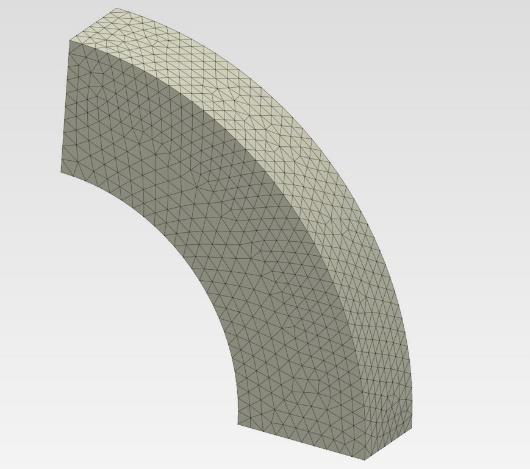
\includegraphics[width=78mm]{fig/01-01.png}
	\caption{分割リング - メッシュ}
	\label{fig:01-01}
	\end{figure}
\item
	境界条件と荷重を適用する際に使用するノードセットfix(下側)とサーフェスpress(上側)を作成します。
\item 
	Steelという名前の新しい材料を定義し、弾性挙動を加え、ヤング率を210000MPa、ポアソン比を0.3と指定します。
	材料にSteelを使用し、Steel\_sectionという名前のソリッドセクションを新規に作成し、そのセクションが割り当てられるように分割リングを選択します。
\item
	デフォルトの設定で静的解析ステップを定義します。
\item
	fixという名前のノードセットに固定境界条件を追加します。
	pressという名前のサーフェスに圧力荷重を追加し、その大きさを20MPaに指定します(図\ref{fig:01-02})。
	\begin{figure}[H]
	\centering
	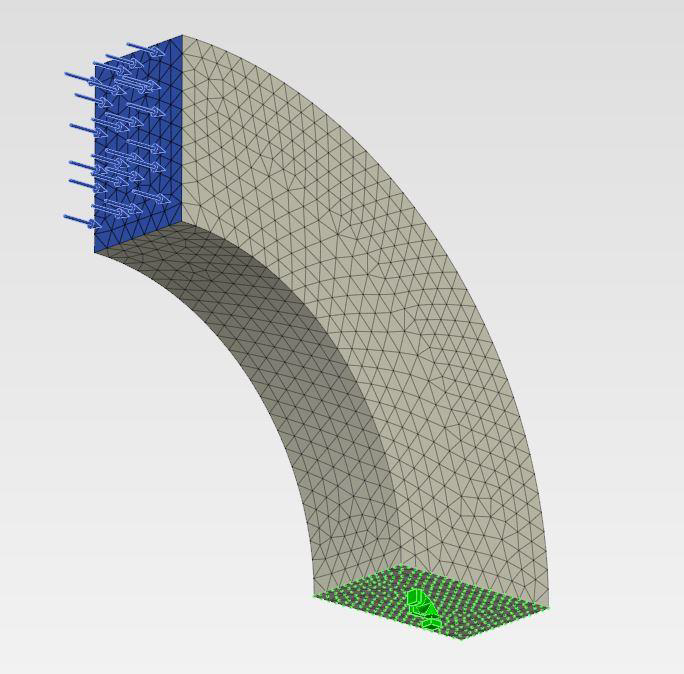
\includegraphics[width=78mm]{fig/01-02.png}
	\caption{分割リング - 境界条件と荷重}
	\label{fig:01-02}
	\end{figure}
\item
  必要な定義がすべて行われたので、解析を提出できます。
  解析が終了するまで待って、結果を開きます。
\item
  ミーゼス応力と変位のコンタープロットを確認します。
  カラースペクトルの種類をRainbowに変更します。
  最大値ラベルを非表示にし、数値フォーマットを一般に変更し、変形スケール係数を40に設定します(図\ref{fig:01-03})。
  分析的に計算された最大応力値は230.68MPaであり、固定面の外側短辺を確認した場合のシミュレーション結果にも同様の応力が見られます。
	\begin{figure}[H]
	\centering
	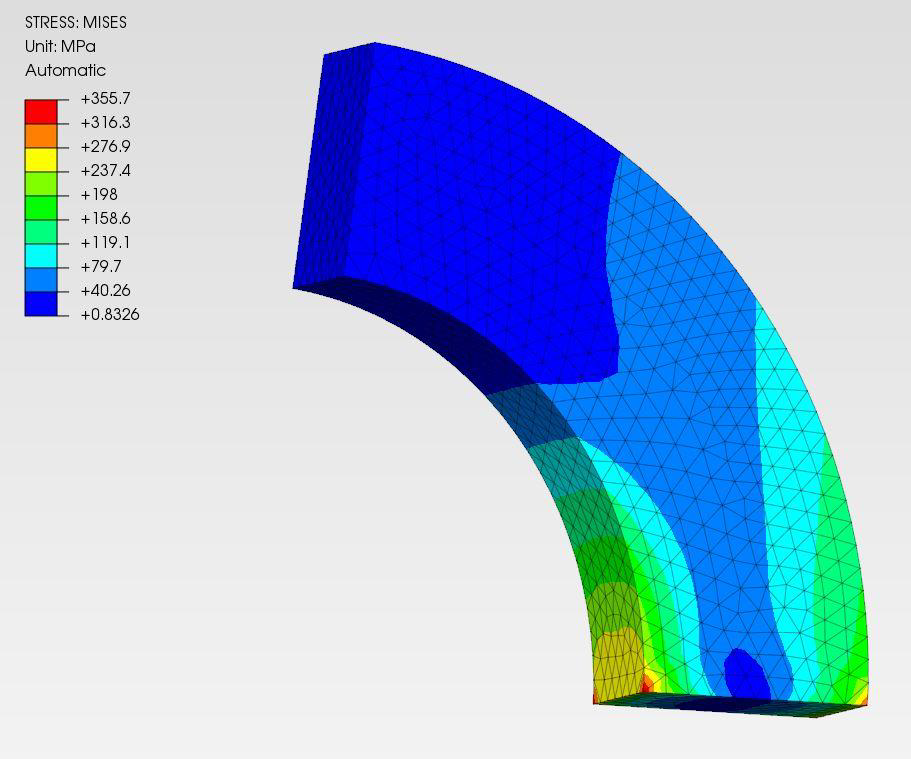
\includegraphics[width=90mm]{fig/01-03.png}
	\caption{分割リング - フォンミーゼス応力}
	\label{fig:01-03}
	\end{figure}
\end{enumerate}
\section{シャフトに表面トラクション荷重}
この例では、短い円形のシャフトに表面トラクション荷重をかけて曲げを発生させます。その寸法は:
\begin{itemize}
\item 直径:50 mm
\item 長さ: 200 mm
\end{itemize}
\begin{enumerate}
\item 
{[}mm, ton, s,  °C{]}単位の新規ファイルを作成し、ステップ形式のジオメトリをPrePoMaxにインポートします。
次に、パーツをメッシュ分割します。
ここでは、最大要素サイズとして4mmを選択し、その他の設定は変更しませんでした(図\ref{fig:02-01})。
	\begin{figure}[H]
	\centering
	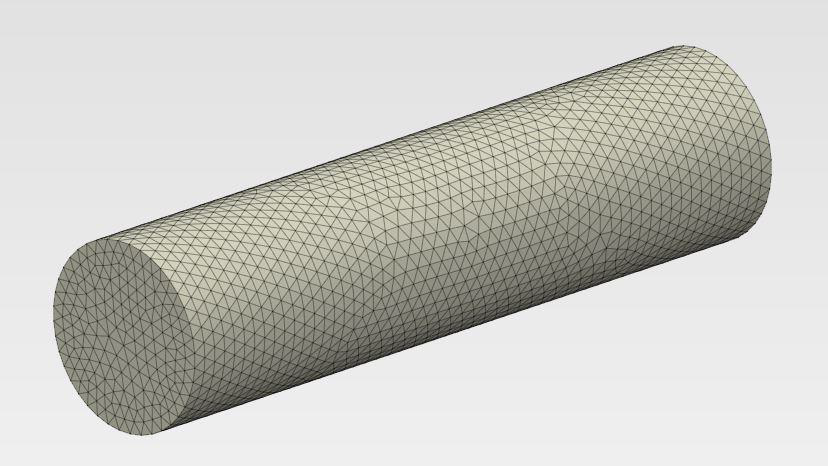
\includegraphics[width=100mm]{fig/02-01.png}
	\caption{シャフト - メッシュ}
	\label{fig:02-01}
	\end{figure}
\item
  新しい材料を定義し、弾性挙動を加え、ヤング率を210000MPa、ポアソン比を0.3と指定します。
  先に作成した材料を参照して新しいソリッドセクションを作成し、そのセクションがこのパーツに割り当てられるようにシャフトを選択します。
\item
  デフォルトの設定で静的解析ステップを定義します。
  固定境界条件をシャフトの片方の端に、表面トラクション荷重を、もう片方の端に割り当てます。
  シャフトの軸に垂直な方向に-500Nの値を指定します(図\ref{fig:02-02})。
	\begin{figure}[H]
	\centering
	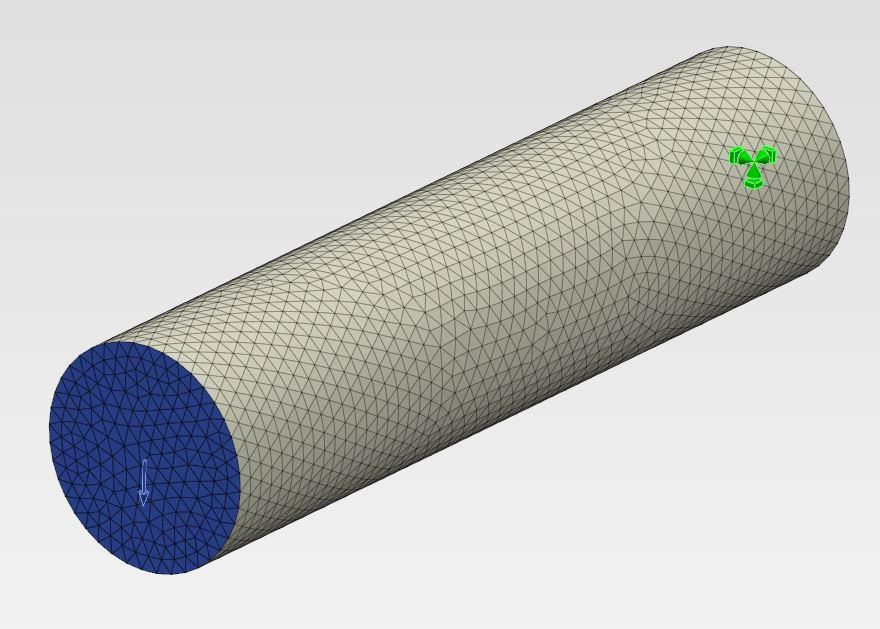
\includegraphics[width=97mm]{fig/02-02.png}
	\caption{シャフト - 境界条件と荷重}
	\label{fig:02-02}
	\end{figure}
\item
  解析を実行し、解析が完了したら結果を開きます。
  変形のスケール係数を400に変更し、非変形モデルを描画するオプションをオンにします。
  変位のコンタープロットを調べ、非変形モデルの形状を隠し、ミーゼス応力のプロットを確認します(図\ref{fig:02-03})。
  分析的に計算された最大応力は8.17MPaで、解析結果を確認しても同様の値が得られます。
	\begin{figure}[H]
	\centering
	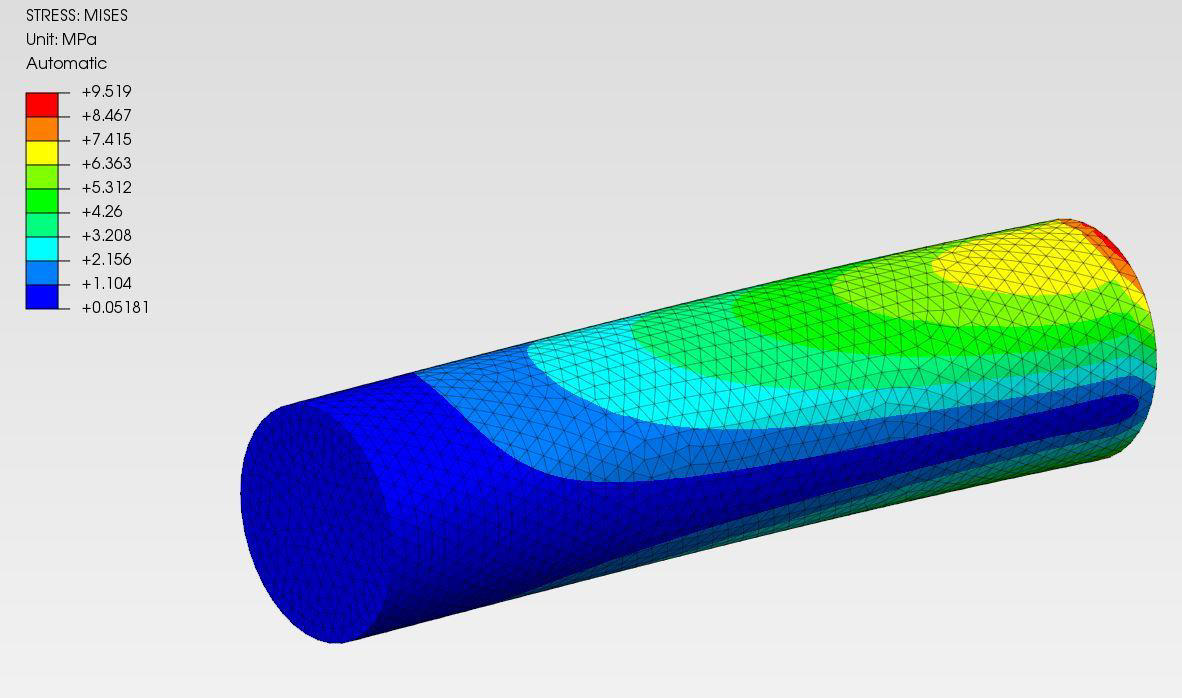
\includegraphics[width=123mm]{fig/02-03.png}
	\caption{シャフト - フォンミーゼス応力}
	\label{fig:02-03}
	\end{figure}
\end{enumerate}
\section{楕円形の棒のねじり}
このケースでは、楕円形の断面を持つ棒にねじりを加えています。その寸法は:
\begin{itemize}
\item 長軸:200mm
\item 短軸:100mm
\item 長さ:1000mm
\end{itemize}
\begin{enumerate}
\item
  {[}mm, ton, s, °C{]}単位の新規ファイルを作成し、ステップ形式のジオメトリをPrePoMaxにインポートします。
  次に、パーツをメッシュ分割します。ここでは、最大要素サイズとして10mmを選択し、その他の設定は変更しませんでした(図\ref{fig:03-01})。
	\begin{figure}[H]
	\centering
	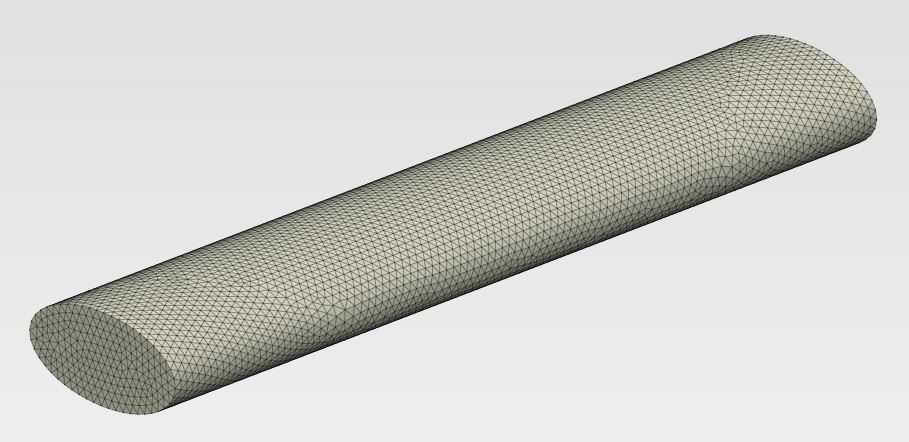
\includegraphics[width=127mm]{fig/03-01.png}
	\caption{楕円形の棒 - メッシュ}
	\label{fig:03-01}
	\end{figure}
\item
  新しい材料を定義し、弾性挙動を加え、ヤング率を210000MPa、ポアソン比を0.3と指定します。
  先に作成した材料を参照して新しいソリッドセクションを作成し、そのセクションがこのパーツに割り当てられるようにシャフトを選択します。
\item
  座標(0, 0, 1000)に基準点を作成します。
  この基準点を使って剛体拘束を作成し、シャフトの表面に割り当てます。
\item
  デフォルトの設定で静的解析ステップを定義します。
  固定境界条件を基準点のある面と反対側のシャフトの面に割り当てます。
  モーメント荷重を作成して基準点に適用し、棒の軸に1000000Nmmの大きさを指定します(図\ref{fig:03-02})。
	\begin{figure}[H]
	\centering
	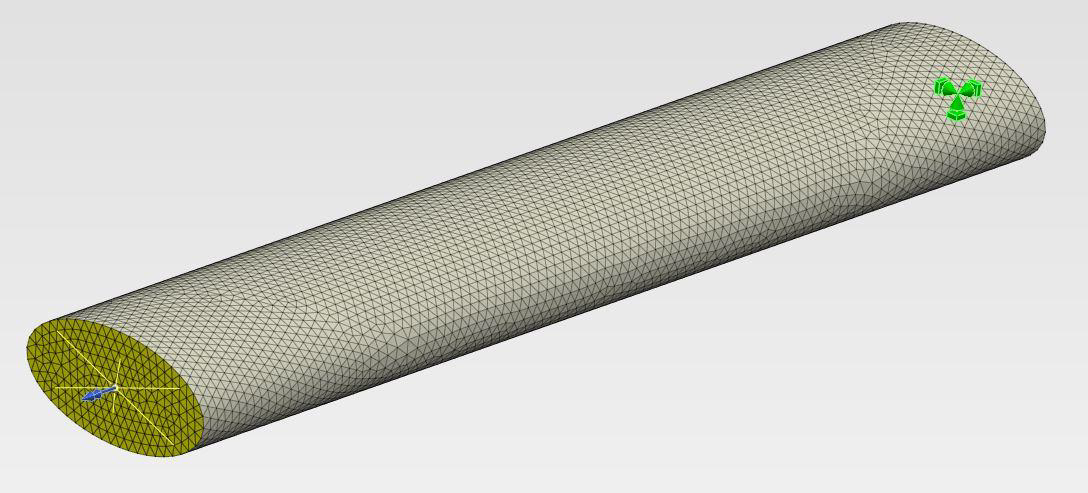
\includegraphics[width=142mm]{fig/03-02.png}
	\caption{楕円形の棒 - 境界条件と荷重}
	\label{fig:03-02}
	\end{figure}
\item
  解析を実行し、解析が完了したら結果を開きます。
  このケースでは、分析的に計算された最大せん断応力は2.547MPaです。
  数値結果と比較するために、適切な応力成分に切り替えます(モデルがグローバル座標系の軸にどのように配置されているかによって異なります)。
  Query → Point/Nodeツールを使って、棒のさまざまな場所の応力値を調べます。
  また、最大せん断応力を持つノードを指すラベルを表示します。
  この場合の結果は2.555MPaで、解析解に非常に近いものでした(図\ref{fig:03-03})。
	\begin{figure}[H]
	\centering
	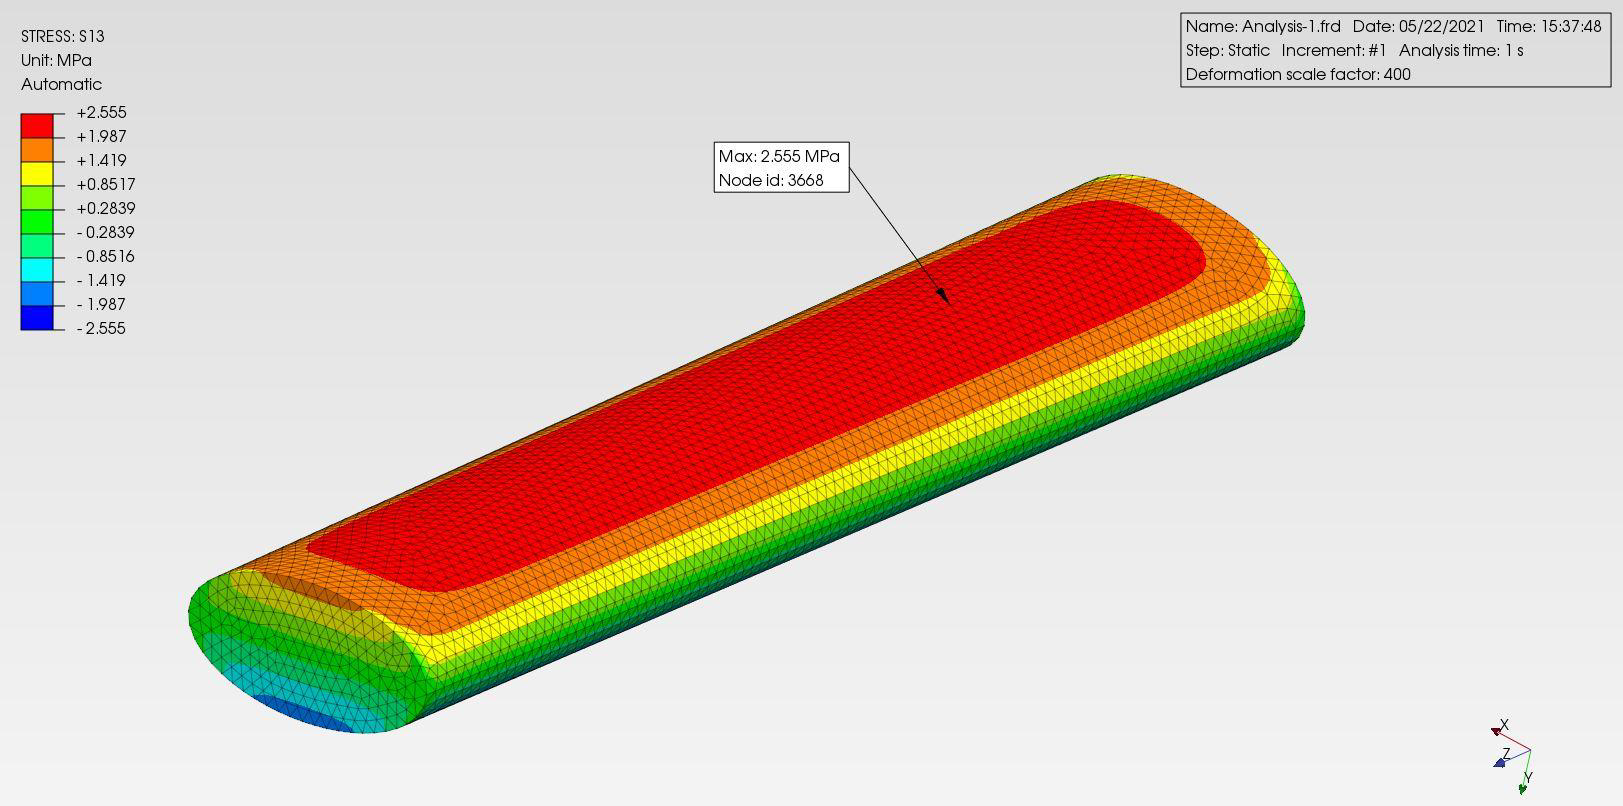
\includegraphics[width=150mm]{fig/03-03.png}
	\caption{楕円形の棒 - せん断応力}
	\label{fig:03-03}
	\end{figure}
\end{enumerate}
\section{ねじりと曲げを受ける長方形の棒}
このケースでは、複合荷重(ねじりと曲げ)を受ける長方形断面の棒を解析します。その寸法は:
\begin{itemize}
\item 断面:200$\times$300mmの長方形
\item 長さ:1400mm
\end{itemize}
\begin{enumerate}
\item
  {[}mm, ton, s, °C{]}単位の新規ファイルを作成し、ステップ形式のジオメトリをPrePoMaxにインポートします。
  次に、パーツをメッシュ分割します。
  ここでは、最大要素サイズとして30mmを選択し、その他の設定は変更しませんでした(図\ref{fig:04-01})。
	\begin{figure}[H]
	\centering
	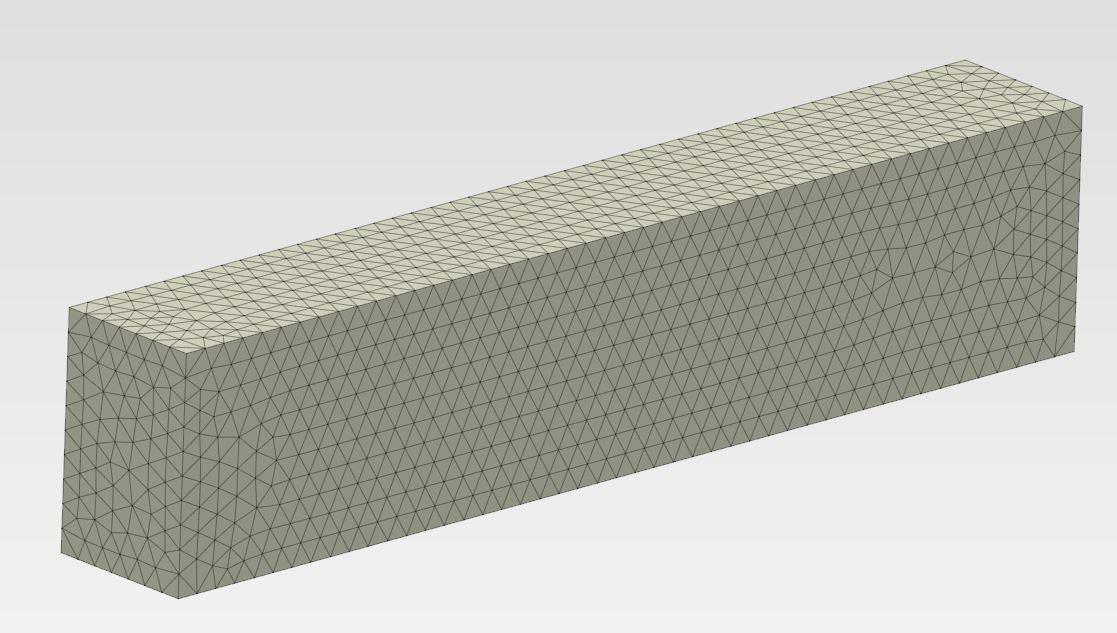
\includegraphics[width=125mm]{fig/04-01.png}
	\caption{長方形の棒 - メッシュ}
	\label{fig:04-01}
	\end{figure}
\vspace{-\baselineskip}
\item
  新しい材料を定義し、弾性挙動を加え、ヤング率を180000MPa、ポアソン比を0.25と指定します。
  先に作成した材料を参照して新しいソリッドセクションを作成し、そのセクションがこのパーツに割り当てられるように棒を選択します。
\item
  座標(500, 0, 1400)に基準点を作成します。
  この基準点を使って剛体拘束を作成し、棒の表面に割り当てます。
\item
  デフォルトの設定で静的解析ステップを定義します。
  固定境界条件を基準点のある方と反対側の棒の端に割り当てます。
  もう一方の棒には集中荷重を設定します。棒の軸に垂直な方向に-8000Nの値を指定します(図\ref{fig:04-02})。
	\begin{figure}[H]
	\centering
	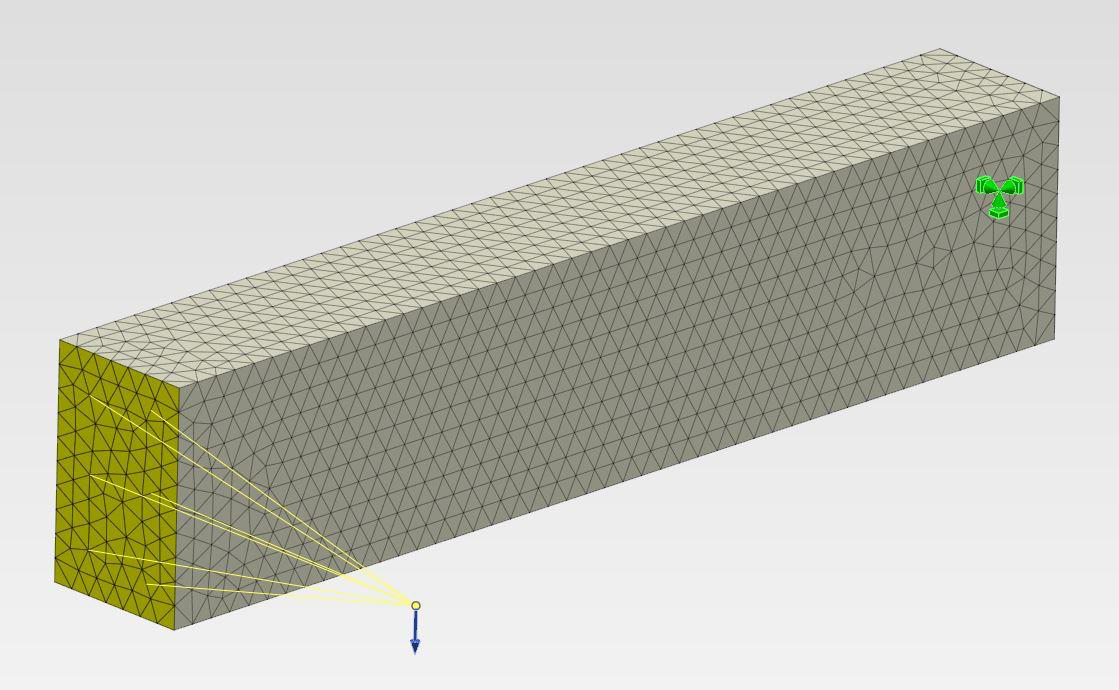
\includegraphics[width=135mm]{fig/04-02.png}
	\caption{長方形の棒 - 境界条件と荷重}
	\label{fig:04-02}
	\end{figure}
\vspace{-\baselineskip}
\item
  解析を実行し、結果を確認します。
  変形のスケール係数を1000に設定し、非変形モデルを描画するオプションを有効にします(図\ref{fig:04-03})。
  リモート荷重によってバーが曲げられたり、ねじられたりしているのがわかります。
  解析結果は4.69MPa程度です。
  シミュレーション結果は応力集中とメッシュ感度の影響を受けますが、この場合、最大応力があるコーナーのすぐ隣のノードで読み取られた値は4.77MPaです。
\vspace{-.5\baselineskip}
	\begin{figure}[H]
	\centering
	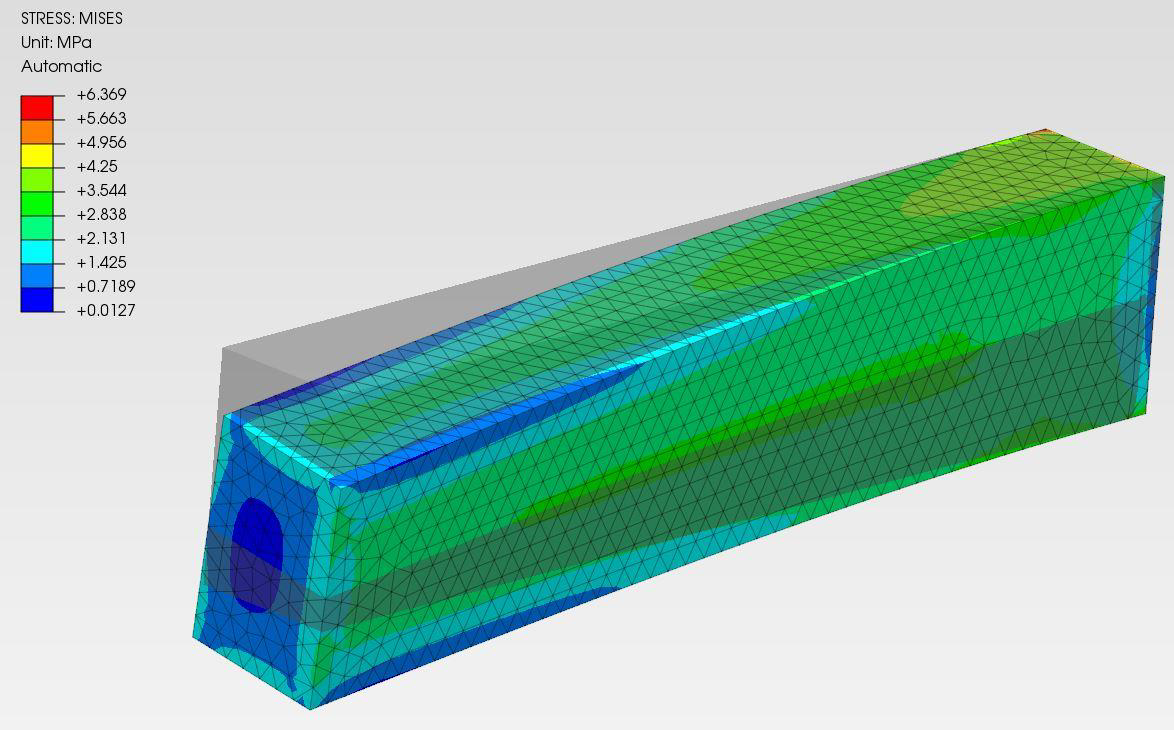
\includegraphics[width=135mm]{fig/04-03.png}
	\caption{長方形の棒 - フォンミーゼス応力}
	\label{fig:04-03}
	\end{figure}
\end{enumerate}
\section{2つの円柱のアセンブリ}
このケースでは、2つの円柱からなる単純なアセンブリを解析します。その寸法は:
\begin{itemize}
\item 1本目の円柱の直径:80mm
\item 1本目の円柱の長さ:100mm
\item 2本目の円柱の直径:50mm
\item 2本目の円柱の長さ:120mm
\end{itemize}
円柱は、CADソフトウェアで個別のパーツとしてモデル化され、そのアセンブリをステップ形式でインポートする必要があります。
\begin{enumerate}
\item
  {[}mm, ton, s, °C{]}単位の新規ファイルを作成し、ステップ形式のジオメトリをPrePoMaxにインポートします。
  次に、両方のパーツをメッシュ分割します。
  ここでは、最大要素サイズとして5mmを選択し、その他の設定は変更しませんでした(図\ref{fig:05-01})。
	\begin{figure}[H]
	\centering
	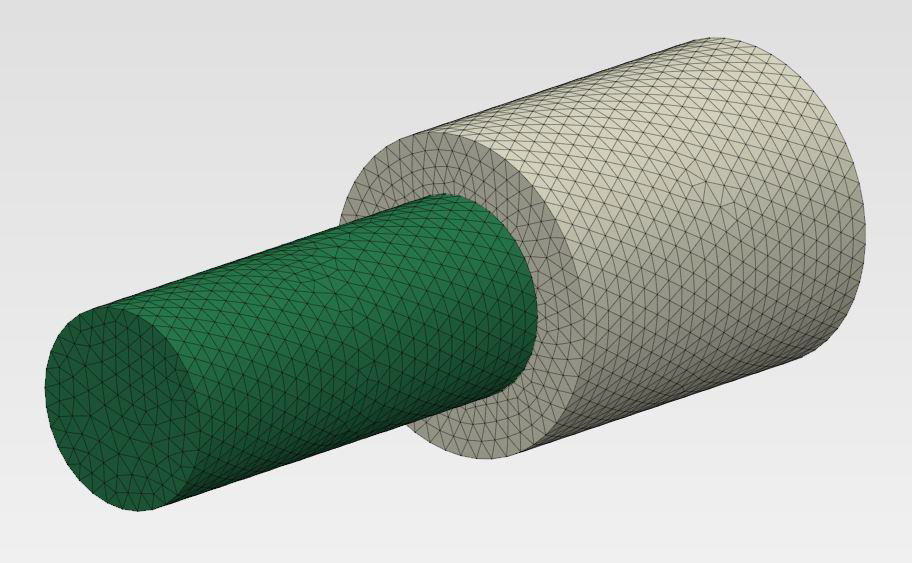
\includegraphics[width=120mm]{fig/05-01.png}
	\caption{2つの円柱 - メッシュ}
	\label{fig:05-01}
	\end{figure}
\vspace{-\baselineskip}
\item
  新しい材料を定義し、弾性挙動を加え、ヤング率を180000MPa、ポアソン比を0.25と指定します。
  先に作成した材料を参照して新しいソリッドセクションを作成し、そのセクションがこのパーツに割り当てられるように円柱を選択します。
\item
  幅の広い円柱を非表示にし、幅の狭い円柱の背面にTie1という名前のサーフェスを作成します。
  パーツの可視性を反転させ(View → Invert Visible Parts)、幅の広い円柱の前面にTie2という名前のサーフェスを作成します。
  再び両方のパーツを表示します。
  タイ拘束を定義し、以前に作成したサーフェスをマスターとスレーブ領域として使用します。
\item
  デフォルトの設定で静的ステップを作成します。
  幅の広い円柱の背面に固定境界条件を適用し、幅の狭い円柱の前面に圧力荷重(大きさ30MPa)を適用します(図\ref{fig:05-02})。
	\begin{figure}[H]
	\centering
	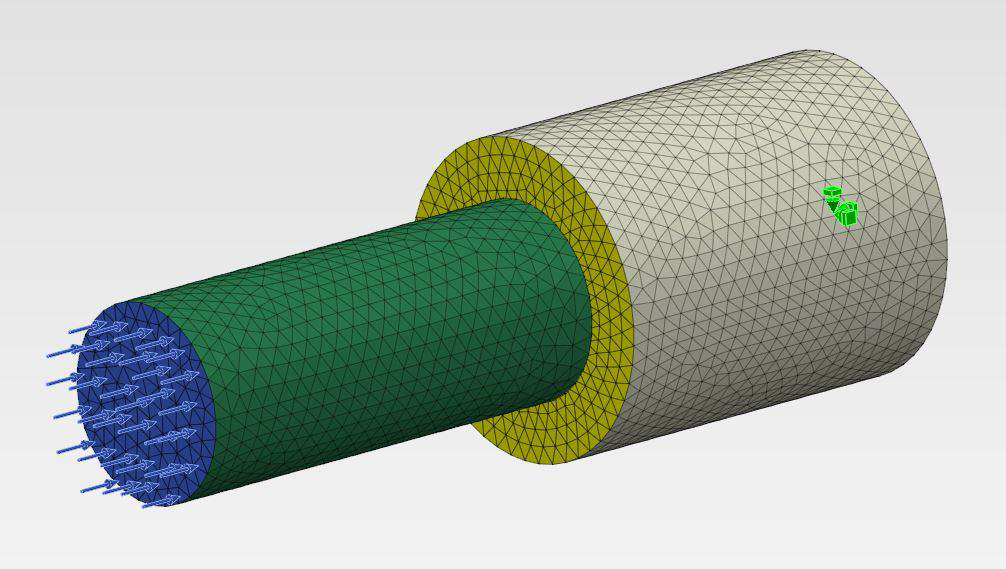
\includegraphics[width=135mm]{fig/05-02.png}
	\caption{2つの円柱 - 境界条件と荷重}
	\label{fig:05-02}
	\end{figure}
\vspace{-\baselineskip}
\item
  解析を実行し、結果を表示します。変形のスケール係数を100として、応力と変位を調べます(図\ref{fig:05-03})。
	\begin{figure}[H]
	\centering
	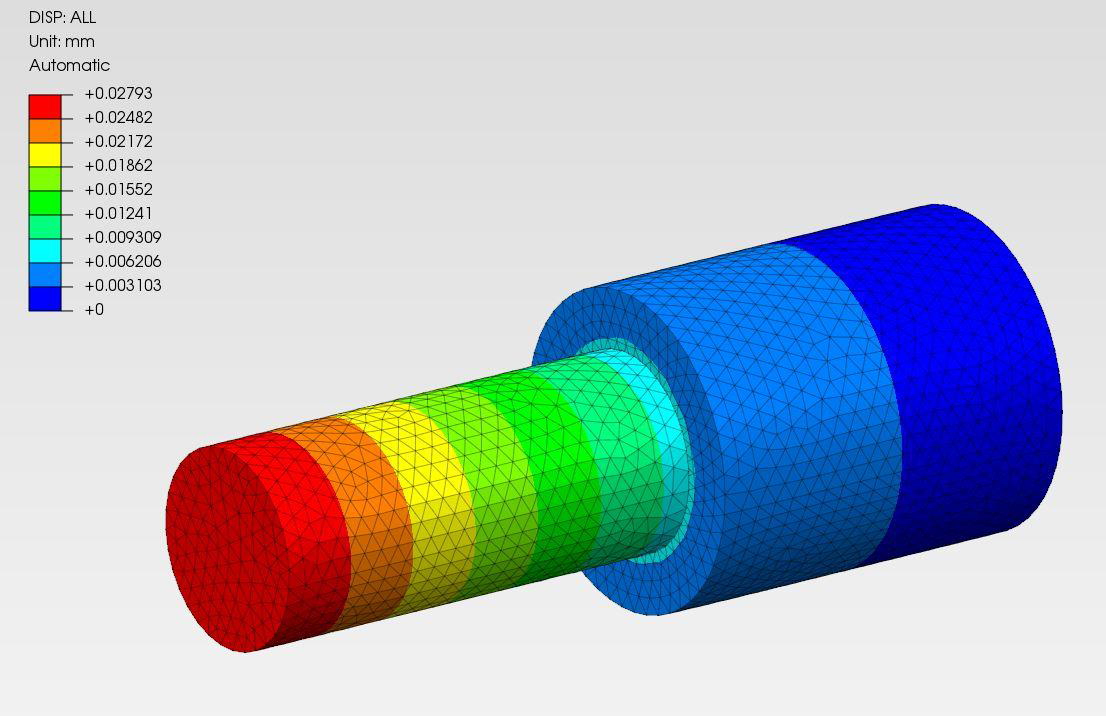
\includegraphics[width=135mm]{fig/05-03.png}
	\caption{2つの円柱 - 変位}
	\label{fig:05-03}
	\end{figure}
\vspace{-\baselineskip}
\end{enumerate}
\section{梁のモーダル解析}
この例では、単純支持された長方形の梁を、固有振動数の観点から解析します。その寸法は:
\begin{itemize}
\item 断面:正方形40 mm
\item 長さ:1000mm
\end{itemize}
\begin{enumerate}
\item
  {[}mm, ton, s, °C{]}単位の新規ファイルを作成し、ステップ形式のジオメトリをPrePoMaxにインポートします。
  次に、パーツをメッシュ分割します。
  ここでは、最大要素サイズとして10mmを選択し、その他の設定は変更しませんでした(図\ref{fig:06-01})。
	\begin{figure}[H]
	\centering
	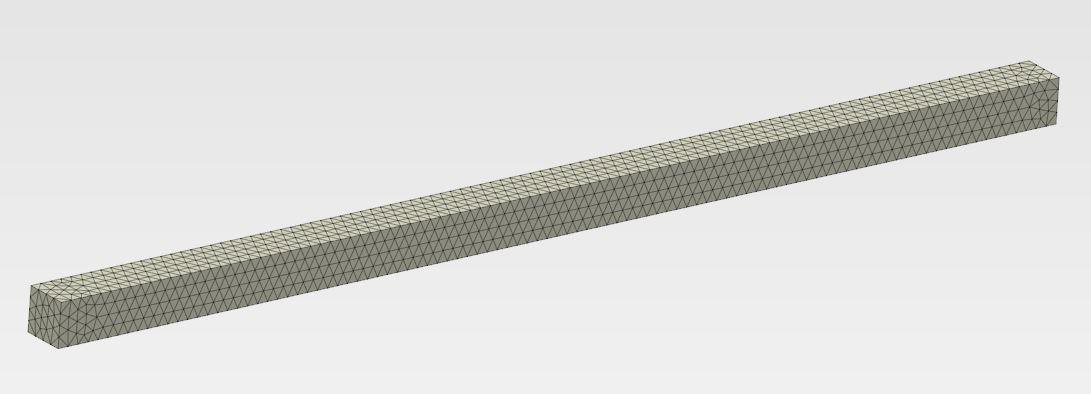
\includegraphics[width=143mm]{fig/06-01.png}
	\caption{梁 - メッシュ}
	\label{fig:06-01}
	\end{figure}
\item
  新しい材料を定義し、弾性挙動を加え、ヤング率を210000MPa、ポアソン比を0.3と指定します。
  また、Density(密度)を追加し、7.85e-9tont/mm3の値を指定します。
  先に作成した材料を参照して新しいソリッドセクションを作成し、そのセクションがこのパーツに割り当てられるように梁を選択します。
\item
  デフォルトの設定で周波数ステップを作成します(10個の固有振動数の抽出)。変位/回転境界条件を一方の端の断面の下部エッジに適用します。
  自由度U1、U2、U3を固定します。
  反対側の断面の下部エッジに適用される別の変位/回転境界条件を作成します。
  先ほどと同様に自由度を固定しますが、ローラー支持をシミュレートするために、1つの移動(ビームの軸方向の移動)を残します(図\ref{fig:06-02})。
	\begin{figure}[H]
	\centering
	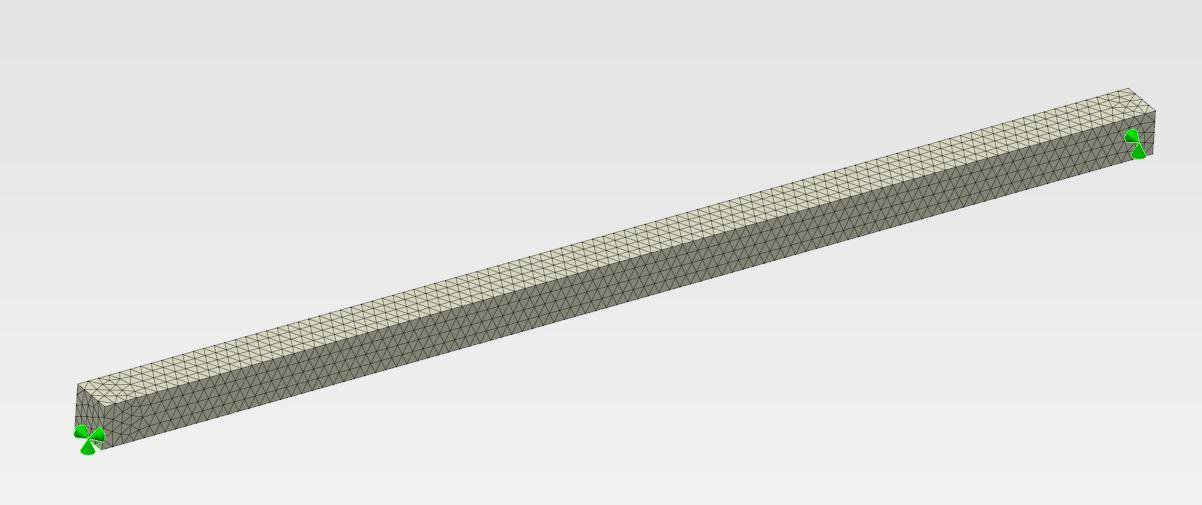
\includegraphics[width=145mm]{fig/06-02.png}
	\caption{梁 - 境界条件}
	\label{fig:06-02}
	\end{figure}
\item
  解析を実行し、解析が完了したら結果を開きます。
  固有振動数とモード形状を調べます。
  モード形状を切り替えるには、Previous/Nextの増分ボタン、またはショートカットツールバーのドロップダウンリストを使用します。
  固有振動数の解析値を以下に示します(表\ref{tab:06-01})。
\end{enumerate}
\begin{table}[H]
\centering
\caption{梁 - 理論固有振動数}
\label{tab:06-01}
\begin{tabular}{|c|c|}
\hline
No. & 固有振動数    \\
    & {[}Hz{]} \\ \hline
1   & 93.82    \\ \hline
2   & 375.46   \\ \hline
3   & 844.07   \\ \hline
4   & 1501.83  \\ \hline
5   & 2347.80  \\ \hline
\end{tabular}
\end{table}
一方、解析で得られた値は次の表(表\ref{tab:06-02})のとおりです。
\begin{table}[H]
\centering
\caption{解析による梁の固有振動数}
\label{tab:06-02}
\begin{tabular}{|c|c|}
\hline
No. & 固有振動数    \\
    & {[}Hz{]} \\ \hline
1 & 93.39\\ \hline
2 & 121.28\\ \hline
3 & 339.68\\ \hline
4 & 413.17\\ \hline
5 & 785.76\\ \hline
6 & 850.47\\ \hline
7 & 1066.7\\ \hline
8 & 1223.69\\ \hline
9 & 1478.86\\ \hline
10 & 1609.22\\ \hline
\end{tabular}
\end{table}
解析計算は簡略化されており(1つの平面内の変形のみを考慮している)、モーダル解析で得られたすべての固有振動数を予測することはできません。これが、この場合の結果の違いの主な理由の1つです。
\vskip\baselineskip
下の画像では、高次モードの形状の1つ(\#9)を見ることができます(図\ref{fig:06-03})。
\begin{figure}[H]
\centering
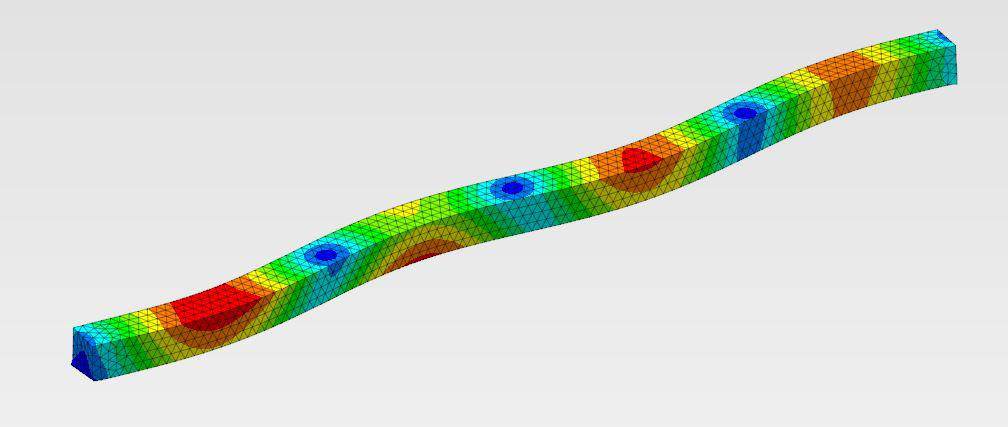
\includegraphics[width=133mm]{fig/06-03.png}
\caption{梁 - モード形状 \#9}
\label{fig:06-03}
\end{figure}
\section{引張弾塑性プレート}
この例では、中央に穴の開いた長方形のプレートに張力をかけています。
プレートは弾塑性材料でできています。対称性のため、プレートの1/4のみを解析します。\\
その寸法は:
\begin{itemize}
\item プレートサイズ:300$\times$150mm
\item 穴の直径:60 mm
\item 厚さ:10 mm
\end{itemize}
\begin{enumerate}
\item
  {[}mm, ton, s, °C{]}単位の新規ファイルを作成し、ステップ形式のジオメトリをPrePoMaxにインポートします。
  次に、パーツをメッシュ分割します。
  ここでは、最大要素サイズとして4mmを選択し、その他の設定は変更しませんでした(図\ref{fig:07-01})。
	\begin{figure}[H]
	\centering
	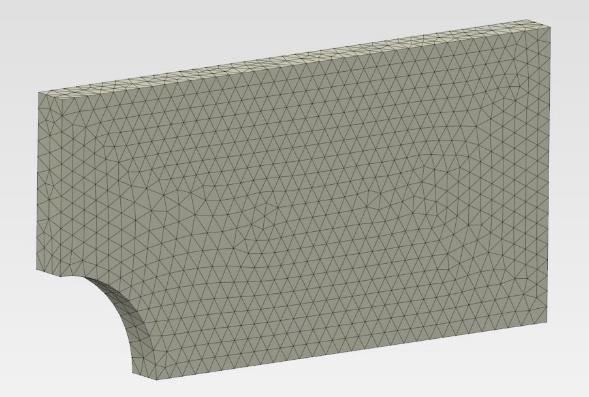
\includegraphics[width=83mm]{fig/07-01.png}
	\caption{プレート - メッシュ}
	\label{fig:07-01}
	\end{figure}
	\vspace{-\baselineskip}
\item
  新しい材料を定義し、弾性挙動を加え、ヤング率を210000MPa、ポアソン比を0.3と指定します。
  また、Plasticity(塑性)を追加し、以下のデータポイントを指定する(表\ref{tab:07-01})。
	\begin{table}[H]
	\centering
	\caption{プレート - 塑性定義のデータポイント}
	\label{tab:07-01}
	\begin{tabular}{|c|c|}
	\hline
	降伏応力 {[}MPa{]} & 塑性ひずみ{[}-{]} \\ \hline
	235 & 0  \\ \hline
	335 & 0.12  \\ \hline
	\end{tabular}
	\end{table}
	\vspace{-\baselineskip}
  先に作成した材料を参照して新しいソリッドセクションを作成し、そのセクションがこのパーツに割り当てられるように梁を選択します。
\item
  デフォルトの設定で静的ステップを定義します。
  対称性のためにカットされた面に変位/回転境界条件を適用します。
  それぞれのBCには、特定の面に垂直な方向に対応する自由度を固定します。
  変位/回転境界条件をもう1つ作成し、もっとも大きい2つの面に適用し、面外変形を防ぐために法線方向の変位を拘束します(実際には問題は2次元です)。
  プレートが引っ張られる側に-200MPaの圧力荷重をかけます(図\ref{fig:07-02})。
	\begin{figure}[H]
	\centering
	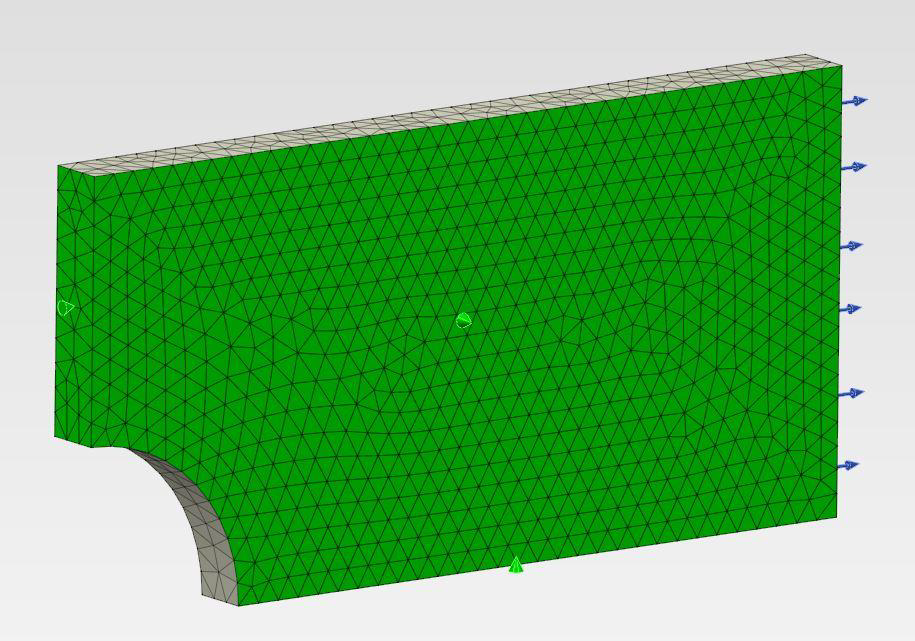
\includegraphics[width=105mm]{fig/07-02.png}
	\caption{プレート - 境界条件}
	\label{fig:07-02}
	\end{figure}
	\vspace{-\baselineskip}
\item
  新しいフィールド出力要求を追加し、要素出力とPEEQ変数を選択します。
\item
  解析を実行し、解析が完了したら結果を確認します。ミーゼス応力と塑性ひずみ(PE)の分布を詳しく見てみましょう(図\ref{fig:07-03})。
	\begin{figure}[H]
	\centering
	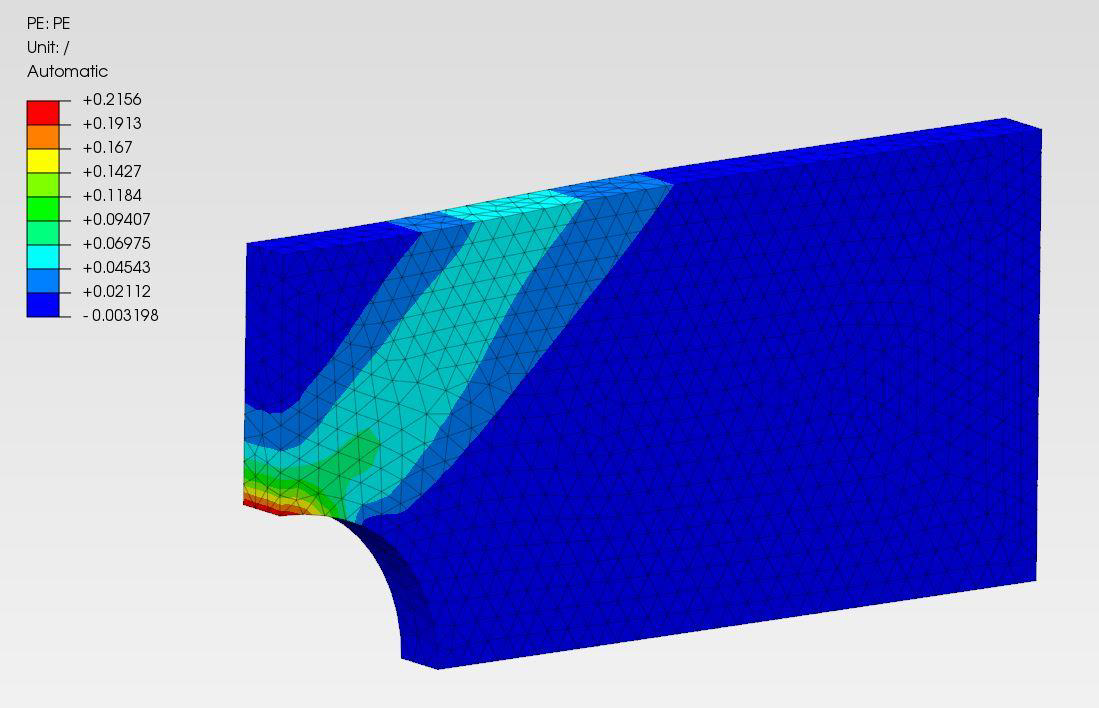
\includegraphics[width=115mm]{fig/07-03.png}
	\caption{プレート - 塑性ひずみ}
	\label{fig:07-03}
	\end{figure}
	\vspace{-\baselineskip}
\item
  Transformation → Symmetryオプションを使用して結果をミラーリングし、プレート全体の結果を表示します(図\ref{fig:07-04})。
	\begin{figure}[H]
	\centering
	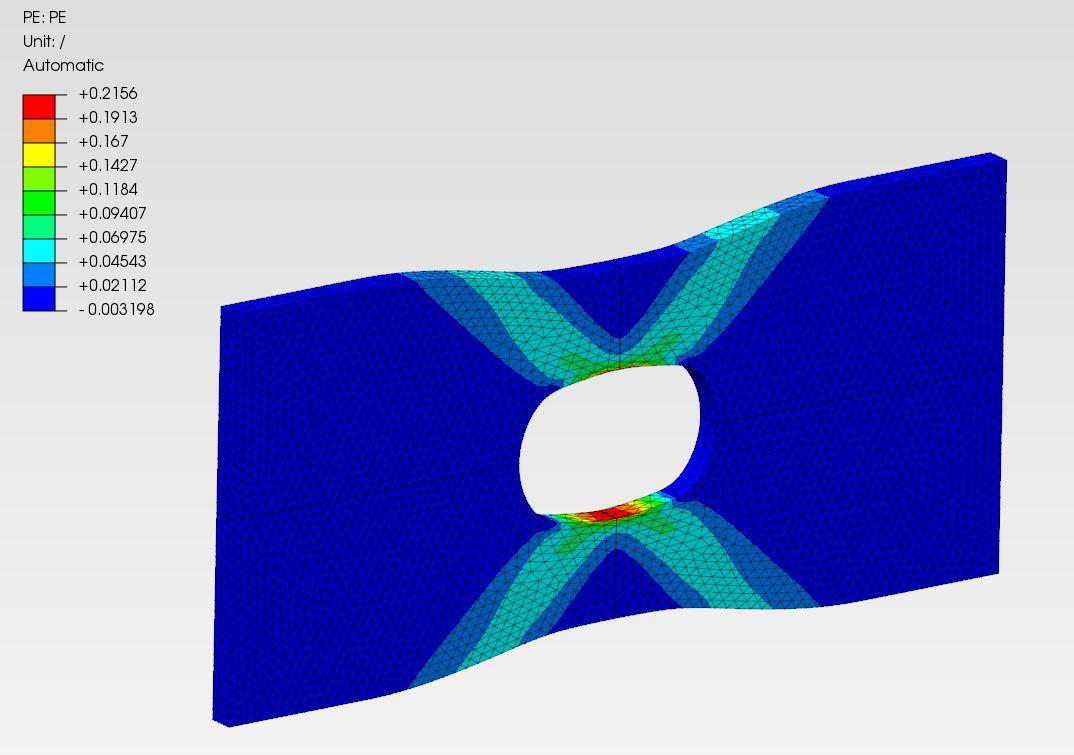
\includegraphics[width=132mm]{fig/07-04.png}
	\caption{プレート - 塑性ひずみ(ミラーリング)}
	\label{fig:07-04}
	\end{figure}
\end{enumerate}
\section{2つの球のヘルツ接触}
ここでは、Code\_Asterのベンチマーク問題SSNV104を例に説明します。
この例では、接触している2つの球体が互いに押し付けられています。
対称性を利用して、それぞれの球体の1/8だけを分析する必要があります。
\vskip.5\baselineskip
ジオメトリは、CADソフトウェアで個別のパーツとしてモデル化され、そのアセンブリをステップ形式でインポートする必要があります。
\begin{enumerate}
\item
  {[}mm, ton, s, °C{]}単位の新規ファイルを作成し、ステップ形式のジオメトリをPrePoMaxにインポートします。
  次に、両方のパーツをメッシュ分割します。
  ここでは、最大要素サイズとして5mmを選択し、その他の設定は変更しませんでした。
  さらに、接触領域に0.5mmの局所的なメッシュ細分化を適用しました(メッシュをより良く細分化するには、球体を分割して、細分化を割り当てることができるエッジを作成する必要があります)。
  そうしないと、ユーザーは接触点の頂点を使用しなければなりません(図\ref{fig:08-01})。
	\begin{figure}[H]
	\centering
	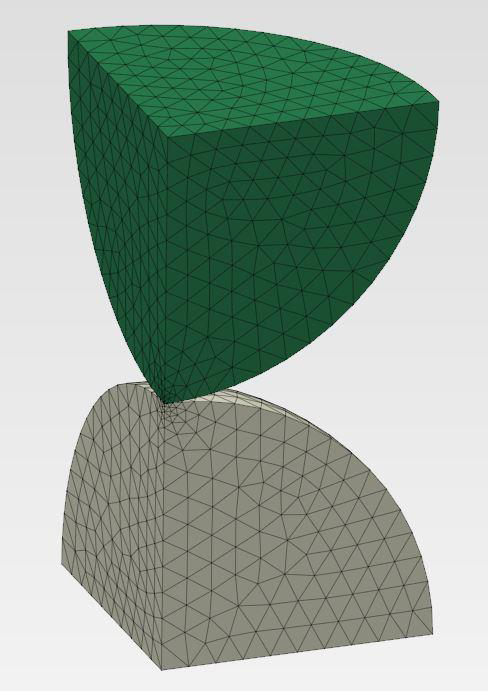
\includegraphics[width=67mm]{fig/08-01.png}
	\caption{2つの球 - メッシュ}
	\label{fig:08-01}
	\end{figure}
\item
  新しい材料を定義し、弾性挙動を加え、ヤング率を20000MPa、ポアソン比を0.3と指定します。
  先に作成した材料を参照して新しいソリッドセクションを作成し、そのセクションがこのパーツに割り当てられるように両方の球セグメントを選択します。
\item
  デフォルトのサーフェス挙動(ハード)でサーフェスの相互作用を作成します。
  この相互作用を参照してコンタクトペアを作成し、解析中に接触する2つのサーフェスを選択します。
\item
  新しい静的ステップを作成し、Nlgeomをオンにします(幾何学的非線形性を考慮するため)。
  2つの変位/回転境界条件を定義し、対称性のある2つの側面からなる2つのセットに適用します(各セットの面の法線方向の変位のみを拘束します)。
  さらに2つの変位/回転境界条件を作成し、上面と下面に割り当てます。
  矢印が互いに向き合い、球が互いに押し付けられるように、2mmと-2mmの変位を規定します(図\ref{fig/08-02.png})。
	\begin{figure}[H]
	\centering
	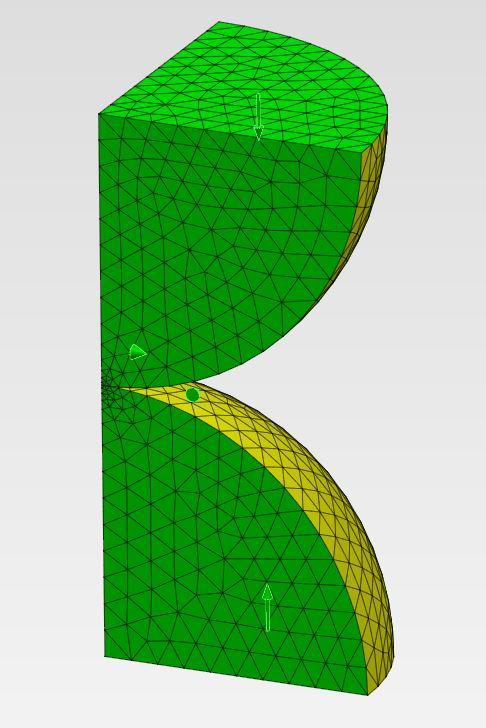
\includegraphics[width=67mm]{fig/08-02.png}
	\caption{2つの球 - 境界条件}
	\label{fig:08-02}
	\end{figure}
\item
  解析を実行し、解析が完了したら結果を確認します。
  接触点の周りの特定の応力分布に注目してください(図\ref{fig:08-03})。
  球体が圧縮される方向(接触点)の法線応力の分析的な計算値は2798.3MPaですが、このケースのシミュレーション結果は2750MPaです。
  接触を伴う解析はメッシュ密度に非常に敏感であるため、メッシュを細かくすることでより良い結果が得られる可能性があります。
	\begin{figure}[H]
	\centering
	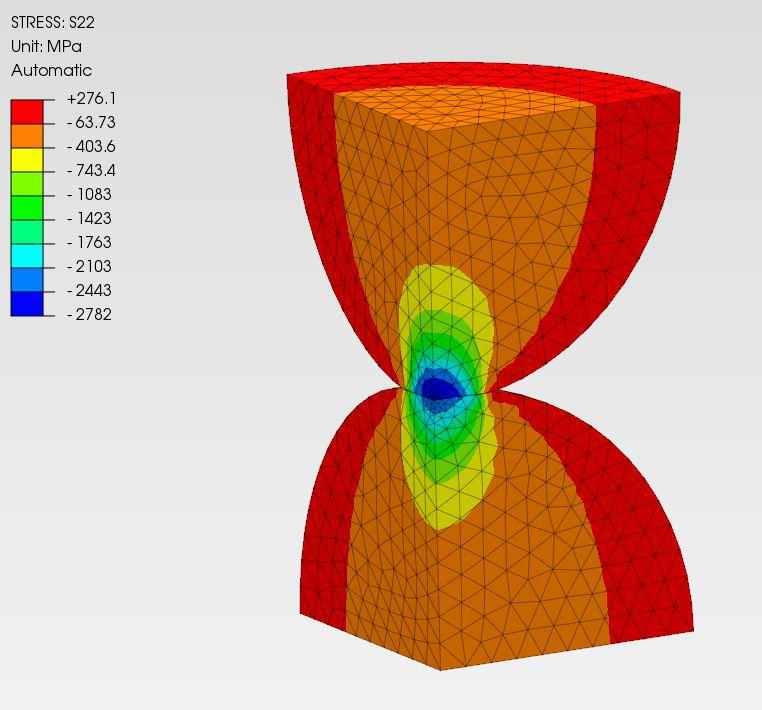
\includegraphics[width=102mm]{fig/08-03.png}
	\caption{2つの球 - 垂直応力}
	\label{fig:08-03}
	\end{figure}
\end{enumerate}
\section{円筒シェルの座屈}
この例では、軸方向に圧縮された円筒形シェルの線形座屈解析を行います。その寸法は:
\begin{itemize}
\item 直径: 300 mm
\item 長さ:600mm
\end{itemize}
ジオメトリーは、CADソフトウェアでサーフェスとしてモデリングされています。
\begin{enumerate}
\item
  {[}mm, ton, s, °C{]}単位の新規ファイルを作成し、ステップ形式のジオメトリをPrePoMaxにインポートします。
  次に、パーツをメッシュ分割します。
  ここでは、最大要素サイズとして10mmを選択し、四分割メッシュを有効にして、その他の設定は変更しませんでした(図\ref{fig:09-01})。
	\begin{figure}[H]
	\centering
	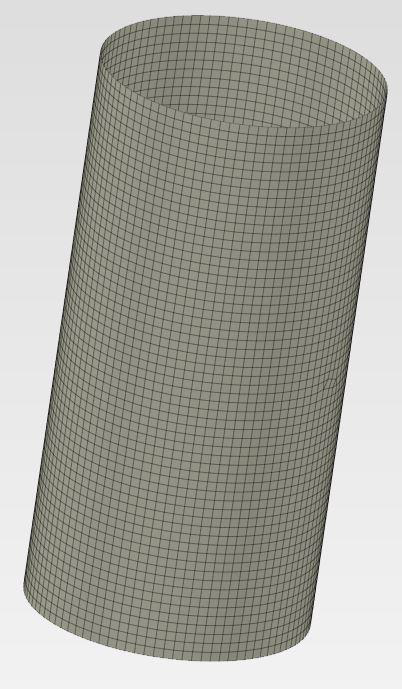
\includegraphics[width=53mm]{fig/09-01.png}
	\caption{円筒シェル - メッシュ}
	\label{fig:09-01}
	\end{figure}
	\vspace{-\baselineskip}
\item
  新しい材料を定義し、弾性挙動を加え、ヤング率を210000MPa、ポアソン比を0.3と指定します。
  先に作成した材料を参照して新しいシェルセクションを作成し、そのセクションがこのパーツに割り当てられるように円筒シェルを選択します。
  厚さを5mmに指定します。
\item
  座標(0, 0, 600)に基準点を作成します。
  この基準点とシェルのエッジを使って剛体拘束を定義します。
\item
  新しい座屈ステップを追加し、座屈係数の数を5に設定します。
  シェルの下部エッジに割り当てられた固定境界条件を作成します。
  集中荷重を定義し、シェルの上端に接続された基準点に適用します。
  この荷重には-1Nを指定します(図\ref{fig:09-02})。
	\begin{figure}[H]
	\centering
	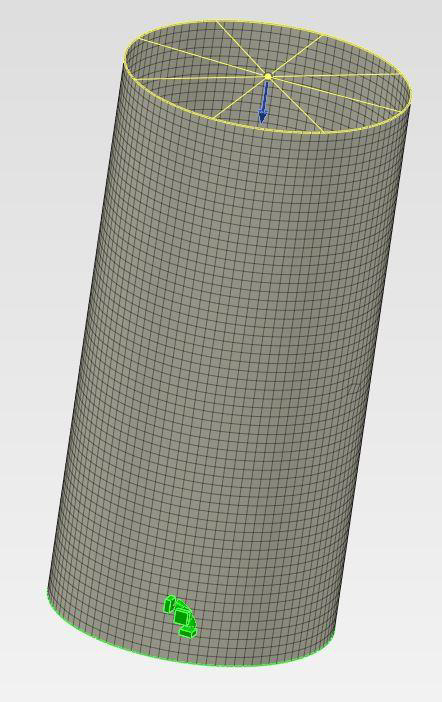
\includegraphics[width=56mm]{fig/09-02.png}
	\caption{円筒シェル - 境界条件と荷重}
	\label{fig:09-02}
	\end{figure}
	\vspace{-\baselineskip}
\item
  解析を実行し、解析が終了したら結果を開きます。
  変形のスケール係数を10000に設定し、座屈モードの形状を確認します。
  そのうちの1つ(\#4)を下の画像に示します(図\ref{fig:09-03})。
  分析的に計算された限界荷重は1.9964-107ですが、シミュレーションでは1.9024-107となります。
	\begin{figure}[H]
	\centering
	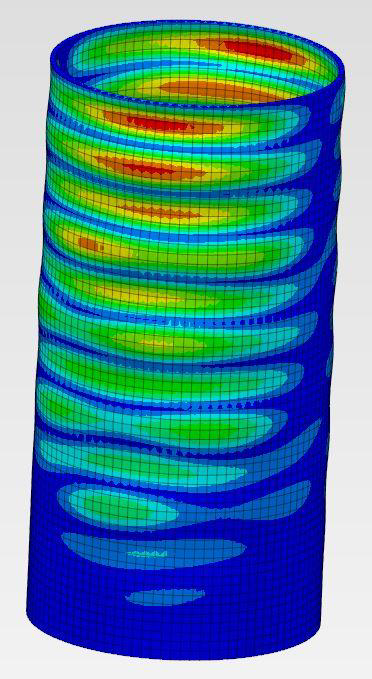
\includegraphics[width=56mm]{fig/09-03.png}
	\caption{円筒シェル - 座屈モード形状 \#4}
	\label{fig:09-03}
	\end{figure}
	\vspace{-\baselineskip}
\end{enumerate}
\section{単純支持されたプレートの圧縮時の座屈}
この例では、単純支持された長方形のプレートのすべての端が圧縮された場合の座屈を解析します。
その寸法は:
\begin{itemize}
\item プレートサイズ:200$\times$150mm
\end{itemize}
ジオメトリーは、CADソフトウェアでサーフェスとしてモデリングされています。
\begin{enumerate}
\item
	{[}mm, ton, s, °C{]}単位の新規ファイルを作成し、ステップ形式のジオメトリをPrePoMaxにインポートします。
	次に、パーツをメッシュ分割します。
	ここでは、最大要素サイズとして5mmを選択し、四分割メッシュを有効にして、その他の設定は変更しませんでした(図\ref{fig:10-01})。
	\begin{figure}[H]
	\centering
	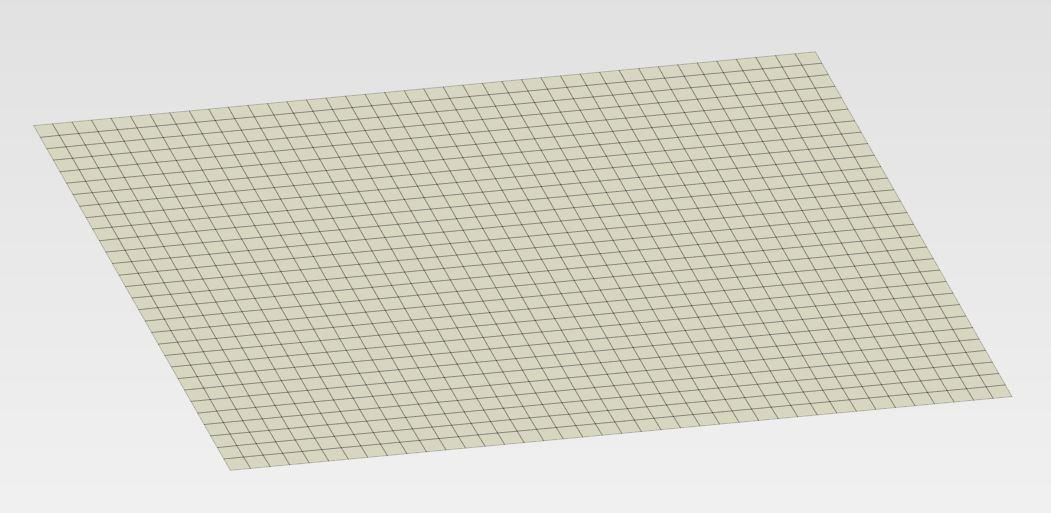
\includegraphics[width=133mm]{fig/10-01.png}
	\caption{プレート - メッシュ}
	\label{fig:10-01}
	\end{figure}
	\vspace{-\baselineskip}
\item
  新しい材料を定義し、弾性挙動を加え、ヤング率を200000MPa、ポアソン比を0.3と指定します。
  先に作成した材料を参照して新しいシェルセクションを作成し、そのセクションがこのパーツに割り当てられるようにプレートを選択します。
  厚さを4mmに指定します。
\item
  新しい座屈ステップを追加し、座屈係数の数を3に設定します。
  プレートのすべてのエッジに割り当てられた変位/回転境界条件を作成し、面外方向の移動のみを拘束します。
  さらに2つの変位/回転境界条件を追加して、プレートの垂直な2つのエッジに適用し、各エッジの法線方向を拘束する。
  法線方向のシェルエッジ荷重を1N/mmの大きさで定義し、法線方向のBCを持つエッジと反対側の2つのエッジに割り当てます(図\ref{fig:10-02})。
	\begin{figure}[H]
	\centering
	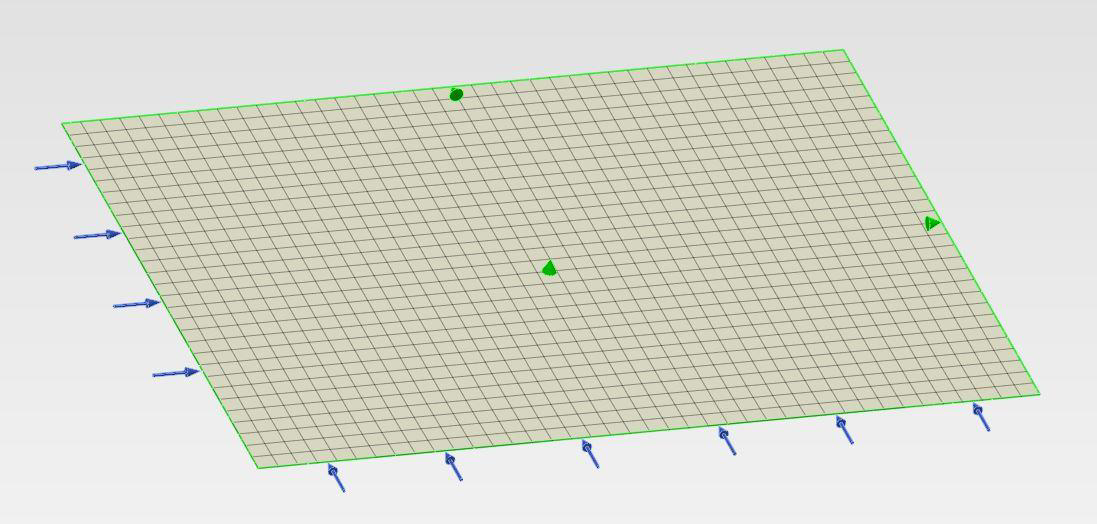
\includegraphics[width=137mm]{fig/10-02.png}
	\caption{プレート - 境界条件と荷重}
	\label{fig:10-02}
	\end{figure}
	\vspace{-\baselineskip}
\item
  解析を実行し、解析が終了したら結果を確認します。
  各座屈モード形状を確認します。2つ目は、下の画像のようになります(図\ref{fig:10-03})。
  分析的に計算した限界圧縮応力は200.85MPaですが、シミュレーションでは197MPaとなります。
	\begin{figure}[H]
	\centering
	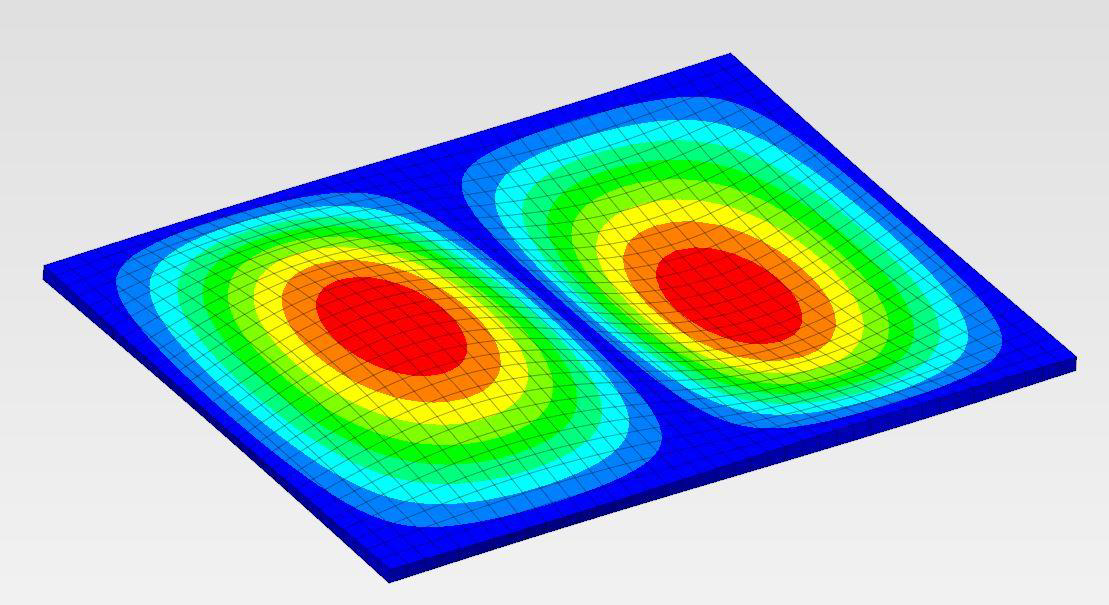
\includegraphics[width=138mm]{fig/10-03.png}
	\caption{プレート - 座屈モード形状 \#2}
	\label{fig:10-03}
	\end{figure}
\end{enumerate}
\section{断熱パイプラインの熱伝達}
この例では、断熱されたパイプラインに熱負荷がかかります。その寸法は:
\begin{itemize}
\item 外径:57 mm
\item 内径: 50 mm
\item 断熱材の厚さ: 28 mm
\item 長さ: 200 mm
\end{itemize}
\begin{enumerate}
\item
  {[}mm, ton, s, °C{]}単位の新規ファイルを作成し、ステップ形式のジオメトリをPrePoMaxにインポートします。
  次に、両方のパーツをメッシュ分割します。
  ここでは、最大要素サイズとして、断熱材は2mm、パイプは3mmを選択しました。その他の設定は変更しませんでした(図\ref{fig:11-01})。
	\begin{figure}[H]
	\centering
	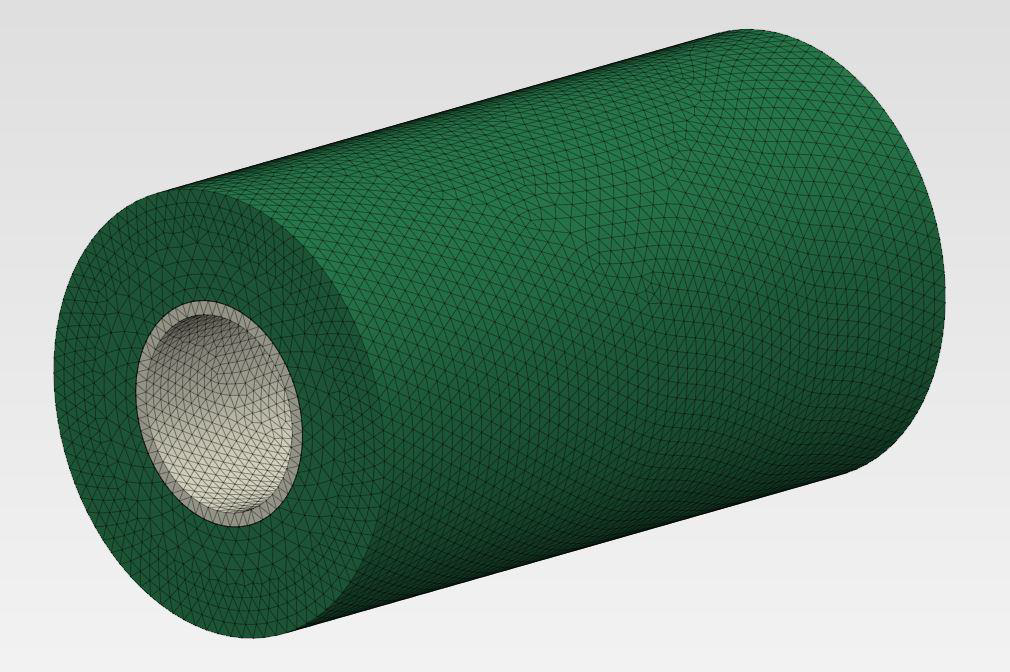
\includegraphics[width=125mm]{fig/11-01.png}
	\caption{パイプライン - メッシュ}
	\label{fig:11-01}
	\end{figure}
	\vspace{-\baselineskip}
\item
  Pipe\_materialという名前の新しいマテリアルを定義し、Thermal conductivity(熱伝導率)を追加して、45mW/(mm-°C)という値を指定します。
  もう1つのマテリアルを定義し、名前をInsulation\_materialとし、Thermal conductivity(熱伝導率)を追加して値を0.05mW/(mm-°C)とします。
  Pipe\_materialを材料として、Pipe\_sectionという名前のソリッドセクションを新規に作成し、そのセクションが割り当てられるように内側のパーツ(パイプ)を選択します。
  別のセクションを作成し、名前をInsulation\_sectionとし、マテリアルとしてInsulation\_materialを選択し、外側のパーツ(断熱材)を選択します。
\item
  パイプを非表示にして、断熱材の内側の面にTie1という名前のサーフェスを作成します。パーツの可視性を反転させ(View → Invert Visible Parts)、パイプの外側の面にTie2という名前のサーフェスを作成します。
  再び両方のパーツを表示します。
  タイ拘束を定義し、以前に作成したサーフェスをマスターとスレーブ領域として使用します。
\item
  熱伝導解析ステップをデフォルト設定(定常状態)で定義します。
\item
  Convective film loadを作成し、断熱材の外表面に割り当てます。
  シンク温度を20°C、熱伝達率を0.015 mW /(mm2・°C)に指定します。
  Convective film loadをもう1つ作成し、パイプの内側表面に割り当てます。
  シンク温度は-30℃、熱伝達率は0.8mW/(mm2-°C)に指定します(図\ref{fig:11-02})。
  	\vspace{-.3\baselineskip}
	\begin{figure}[H]
	\centering
	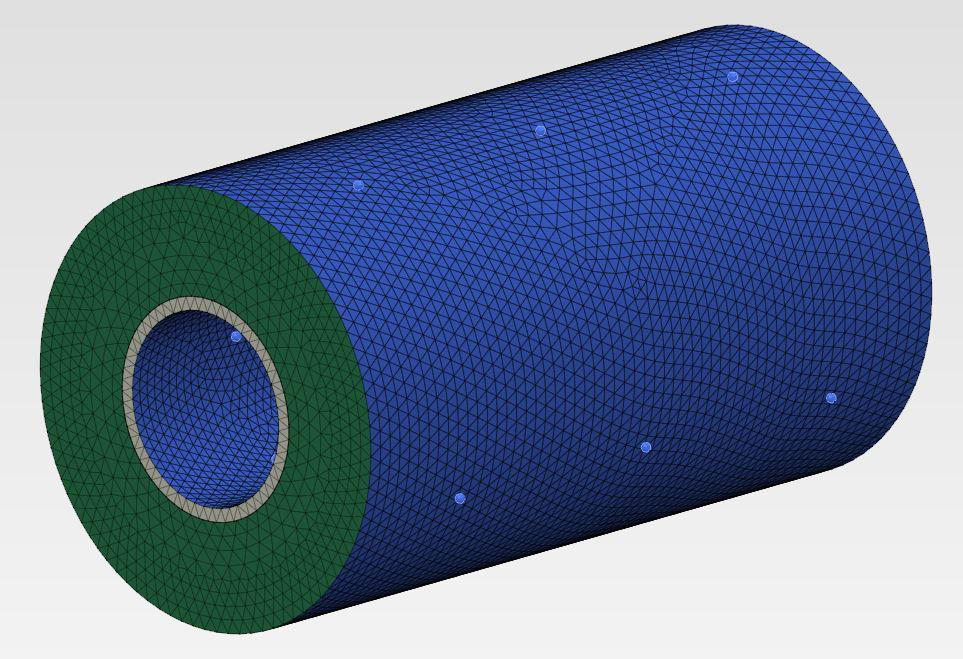
\includegraphics[width=104mm]{fig/11-02.png}
	\caption{パイプライン - 熱負荷}
	\label{fig:11-02}
	\end{figure}
	\vspace{-\baselineskip}
\item
  必要な定義がすべて行われたので、解析を提出できます。
  解析が終了するまで待って、結果を開きます。
\item
  温度コンタープロットを調べます(図\ref{fig:11-03})。
  分析的に計算されたパイプの内側の面の温度は-29.83℃で、パイプの外側の面の温度は16.05℃です。
  同様の値は解析でも確認できます(Query toolで確認してください)。
  	\vspace{-.3\baselineskip}
	\begin{figure}[H]
	\centering
	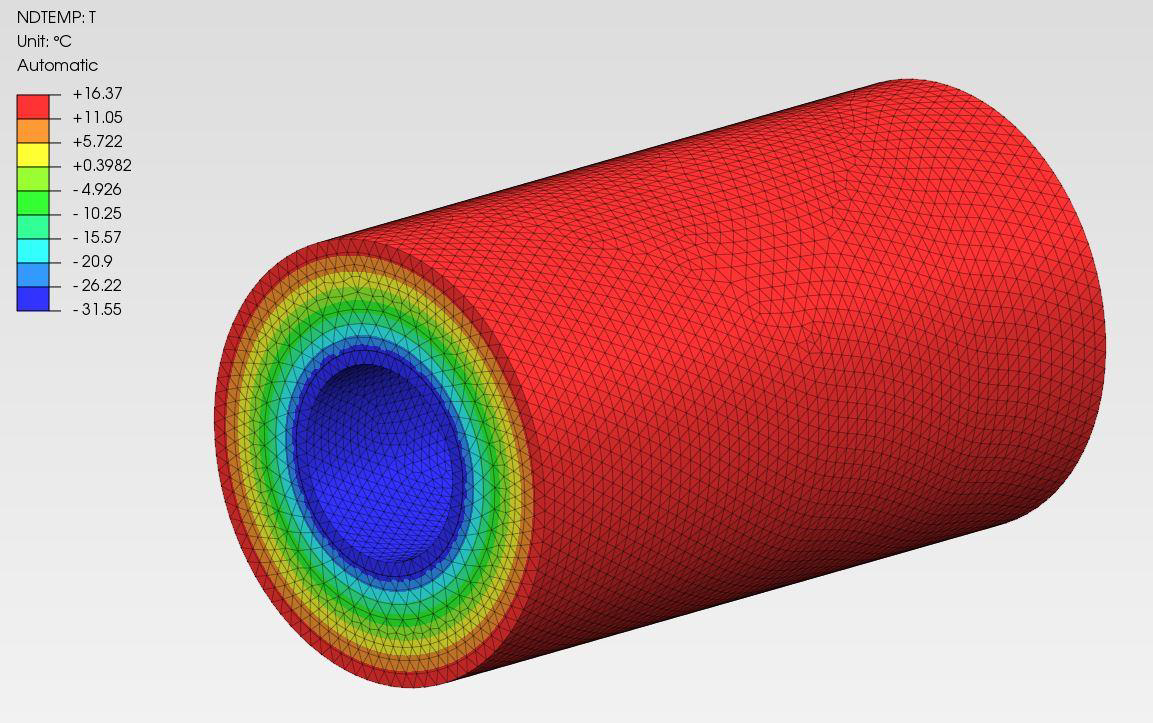
\includegraphics[width=128mm]{fig/11-03.png}
	\caption{パイプライン - 温度}
	\label{fig:11-03}
	\end{figure}
	\vspace{-\baselineskip}
\end{enumerate}
\section{バイメタル小片の熱構造解析}
この例では、バイメタルの小片が、各層の異なる熱膨張のために曲がります。
モデルは、2本の梁(120$\times$20$\times$4mm)を互いに重ねて配置したもので構成されています。
\begin{enumerate}
\item
  {[}mm, ton, s, °C{]}単位の新規ファイルを作成し、ステップ形式のジオメトリをPrePoMaxにインポートします。
  次に、両方のパーツをメッシュ分割します。
  ここでは、両方のパーツの最大要素サイズを1mmとし、その他の設定は変更しませんでした(図\ref{fig:12-01})。
	\begin{figure}[H]
	\centering
	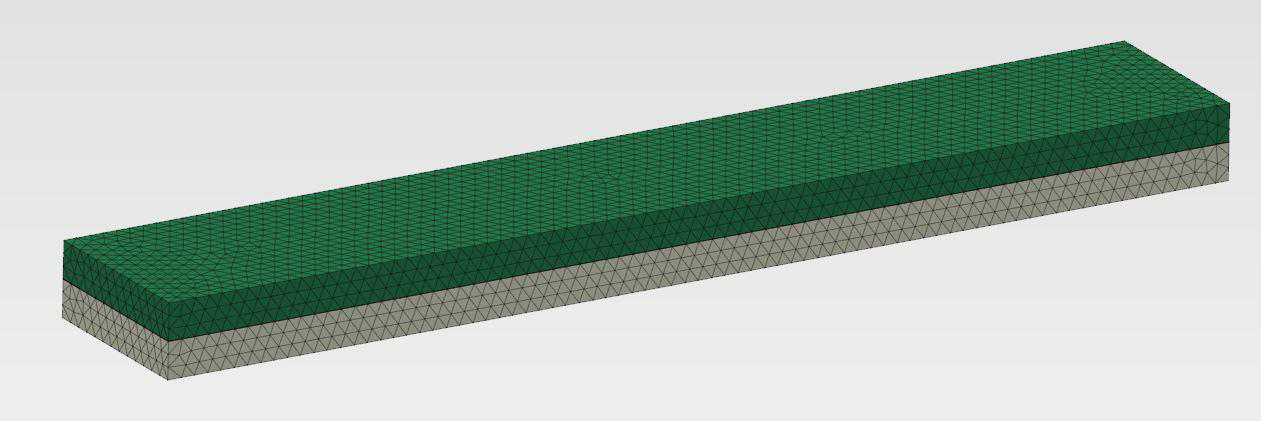
\includegraphics[width=145mm]{fig/12-01.png}
	\caption{バイメタル小片 - メッシュ}
	\label{fig:12-01}
	\end{figure}
	\vspace{-\baselineskip}
\item
  Copperという名前の新しい材料を定義し、弾性(ヤング率130000MPa、ポアソン比0.34)、熱伝導率(385mW/(mm・°C))、熱膨張率(17e-6(1/°C)、零温度20°C)を追加します。
  別の材料を定義し、名前をSteelとし、弾性(ヤング率21000MPa、ポアソン比0.3)、熱伝導率(45mW/(mm・°C))、熱膨張率(12.3e-6(1/°C)、零温度20°C)を追加します。
  材料にCopperを使用し、Top\_layerという名前のソリッドセクションを新規に作成し、そのセクションが割り当てられるように上部の梁を選択します。
  別のセクションを作成し、名前をBottom\_layerとし、材料にSteelを選び、下の梁を選択します。
\item
  上部の梁を非表示にし、下部の梁の上面にTie1という名前のサーフェスを作成します。
  パーツの可視性を反転させ(View → Invert Visible Parts)、上部梁の下面にTie2という名前のサーフェスを作成します。
  再び両方のパーツを表示します。
  タイ拘束を定義し、以前に作成したサーフェスをマスターとスレーブ領域として使用します。
\item
  温度-変位連成解析ステップをデフォルト設定(定常状態)で定義します。
\item
  両方の梁の背面に固定境界条件を割り当てます。
  固定された面以外のすべての外面に、80℃の温度境界条件を追加します(図\ref{fig:12-02})。
	\begin{figure}[H]
	\centering
	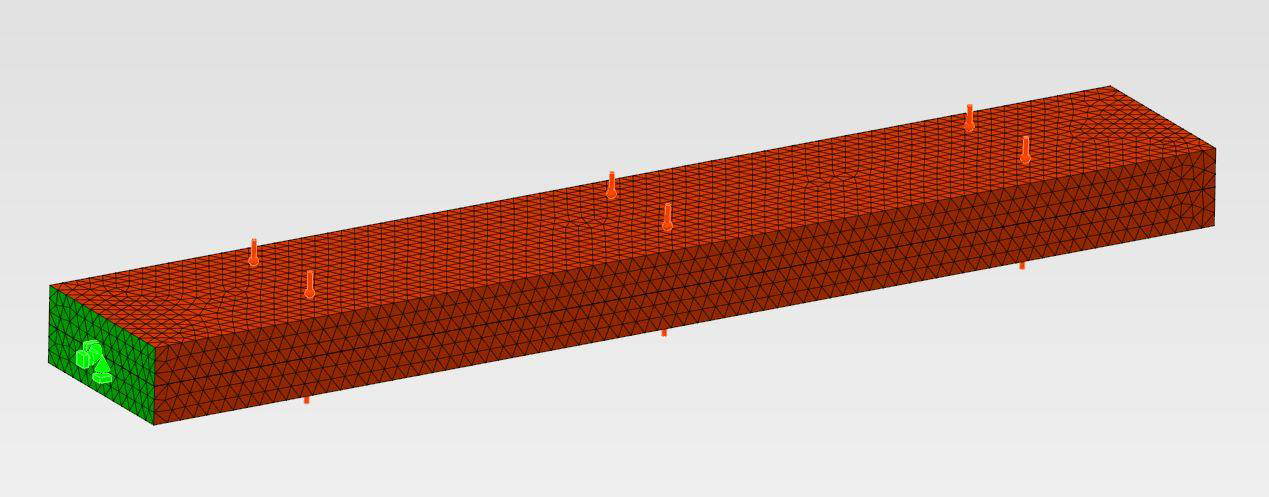
\includegraphics[width=140mm]{fig/12-02.png}
	\caption{バイメタル小片 - 境界条件}
	\label{fig:12-02}
	\end{figure}
	\vspace{-\baselineskip}
\item
  必要な定義がすべて行われたので、解析を提出できます。
  解析が終了するまで待って、結果を開きます。
\item
  垂直変位のコンタープロットを調べます(図37)。
  分析的に計算されたバイメタル小片のたわみは0.3807mmです。
  解析では、これよりも若干高い予測値が得られることがあります。
	\begin{figure}[H]
	\centering
	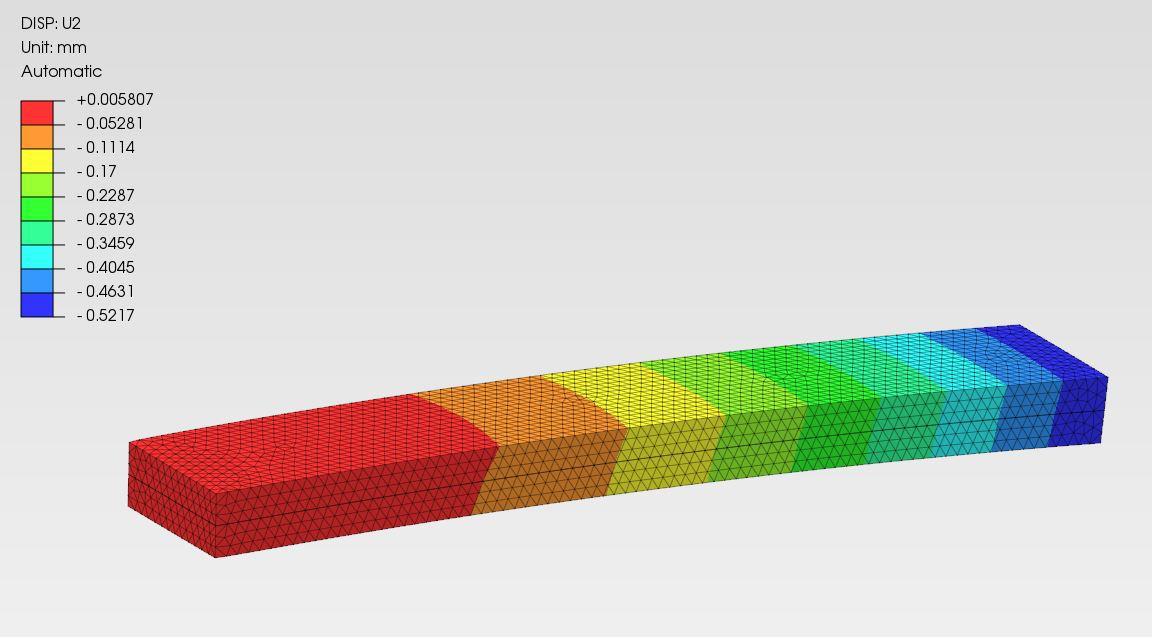
\includegraphics[width=145mm]{fig/12-03.png}
	\caption{バイメタル小片 - たわみ}
	\label{fig:12-03}
	\end{figure}
\end{enumerate}
%
\end{document}
